\section{EmporioLambda Architecture}
EmporioLambda uses 2 different modules:
\begin{itemize}
\item Front-end: module that manages the UI and the user interactions;
\item Back-end: module that manages the data processing, specifically where it is kept and how it is used.
\end{itemize}
This makes it possible for business logic and presentation logic to work separately.

\subsection{Front-end module architecture}
In this section is shown how the Front-end module of EmporioLambda works. In particular it will be explained the role of every part of it.\\The Front-end module can be summarized in 4 primary parts:
\begin{itemize}
\item data pre-fetching: managed with Next.js;
\item components: managed with React;
\item services: functions that communicate with Back-end module;
\item types: classes and data types used.
\end{itemize} 
How these parts communicate each other is illustrated in the image below:
\begin{figure}[H]
\centering
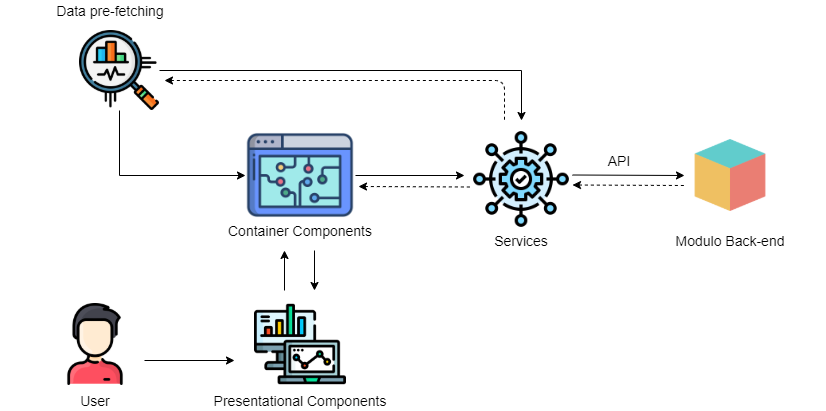
\includegraphics[scale=0.58]{res/Architettura/Frontend/img/general_frontend}\\
\caption{Front-end module general scheme}
\end{figure}



\newpage
\subsubsection{Data prefetching}
The data prefetching on \textit{EmporioLambda} makes use of Next.js pre-rendering.\\
More precisely, Next.js allows the use of 2 types of pre-rendering:
\begin{itemize}
\item \textbf{static generation:} the system generates the HTML at build time. The pre-rendered HTML is then reused on each request;
\begin{figure}[H]
\centering
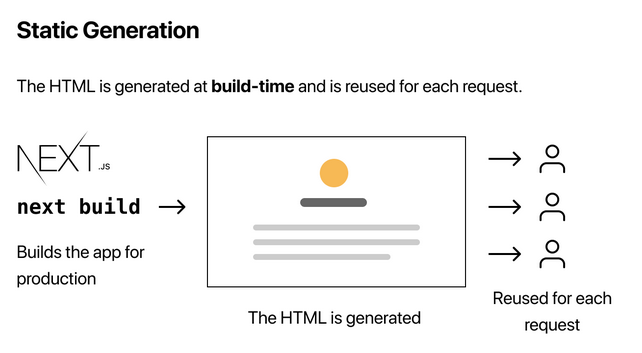
\includegraphics[scale=0.70]{res/Architettura/Frontend/img/staticGeneration}\\
\caption{Static generation scheme}
\end{figure}
\vspace{0.7cm}
\item \textbf{server-side rendering:} the system generates the HTML on each request.
\begin{figure}[H]
\centering
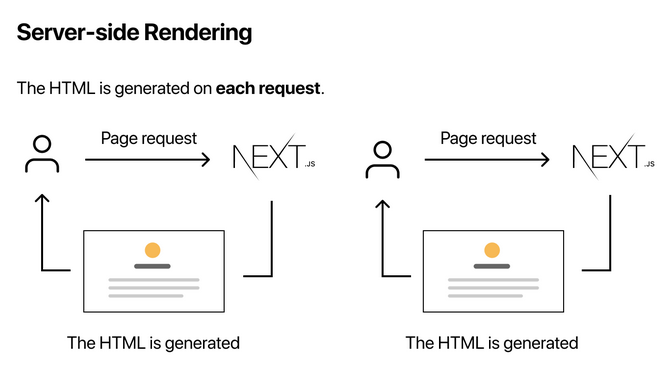
\includegraphics[scale=0.70]{res/Architettura/Frontend/img/serverSideRendering}\\
\caption{Server-side generation scheme}
\end{figure}
\vspace{0.7cm}
\end{itemize}
One difference between these 2 pre-rendering methods is the response time of the website.
Static generation is faster than server-side rendering so the second one should only be used when necessary. Each page can use a different type of prefetch.\\
In \textit{EmporioLambda} each page prefetches data using these 2 methods:
\begin{itemize}
\item \textbf{getStaticProps:} a function that returns a GetStaticProps object, which indicates that the page will use static generation;
\item \textbf{getServerSideProps:} a function that return a GetServerSideProps object, which indicates that the page will use server-side rendering. It will thus render again after receiving new data.
\end{itemize}
Both functions return a Typescript object called props which contains the needed data. This object will be passed to the component part of the Front-end module.\\
More information about Next.js pre-rendering can be found on this page:\\
\url{https://nextjs.org/learn/basics/data-fetching/two-forms}.\\
All of the pages in \textit{EmporioLambda} use server-side rendering.
\newpage
\subsubsection{Components}
To manage the components, EmporioLambda uses React, a Javascript\textsubscript{G} and Typescript\textsubscript{G} library. This allows us to create user-interfaces and UI components.
There are 2 main types of components:
\begin{itemize}
\item \textbf{Presentational Components:} they don't use any state or function. Their only purpose is to show data or call functions from higher level components. Every presentational component can only have children of the same type;
\item \textbf{Container Components:} they can use state variables and functions for their management. They also don't have any restriction about the type of their children.
\end{itemize}
The use of these 2 different components introduces us to the first design pattern used by EmporioLambda: the presentational and container components pattern. This pattern allows us to create a page by using only single components, each with their own responsibility. This also easily lets us separate the \textit{presentational logic} and the \textit{business logic} of the software.\\
React container components can accept 2 variables on their creation:
\begin{itemize}
\item \textbf{props:} variables or objects that can be passed upon component creation by other components;
\item \textbf{state:} variables whose change cause the component to re-render. Its value must be initialized from the component constructor and is read-only.
\end{itemize}
Presentational components can only accept the props variable.\\
The use of the state variables introduces the second design pattern used by EmporioLambda: the observer pattern. This pattern isn't manually implemented by us, as it is a native React pattern. In our case the state of the component is our \textit{observable}: the component, when the state has been changed, automatically re-renders the page with the new values, re-rendering its children as well.\\More information about the observer pattern can be found on this page:\\
\url{https://en.wikipedia.org/wiki/Observer_pattern}.\\

The following diagrams will show the structure of every page, adapted to the UML syntax. The presentational and container components will be recognized by their colors: blue for the first, red for the latter. 

\begin{figure}[H]
\centering
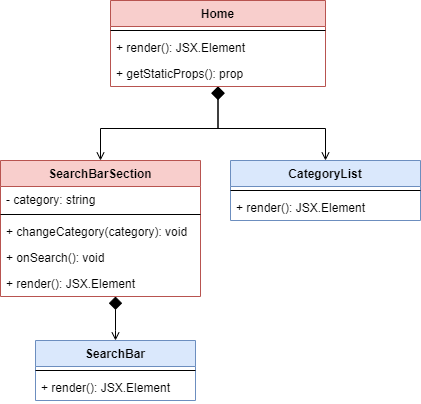
\includegraphics[scale=0.50]{res/Architettura/Frontend/img/home}\\
\caption{Front-end\textsubscript{G} homepage component diagram}
\end{figure}

\begin{figure}[H]
\centering
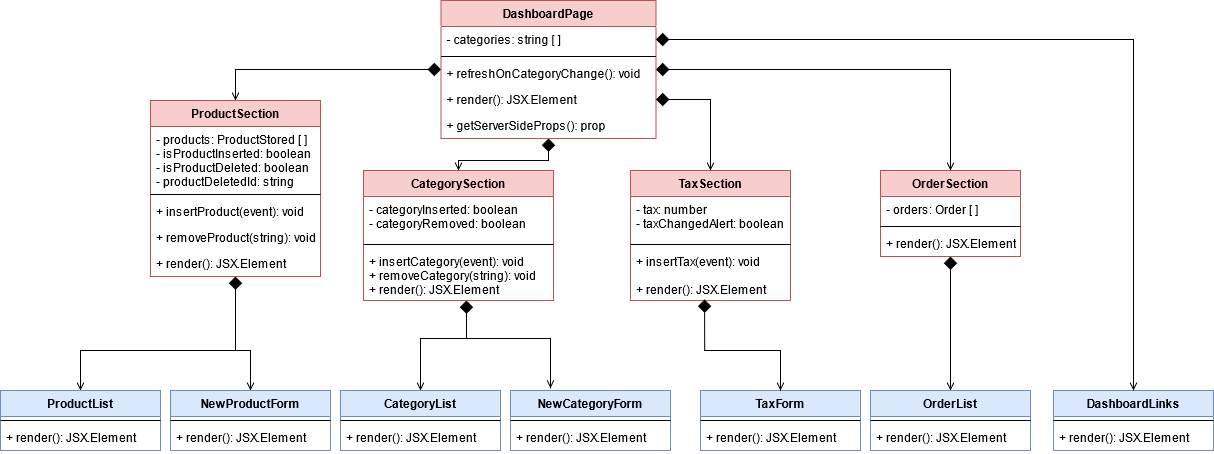
\includegraphics[scale=0.50]{res/Architettura/Frontend/img/dashboard}\\
\caption{Front-end\textsubscript{G} dashboard page component diagram}
\end{figure}

\begin{figure}[H]
\centering
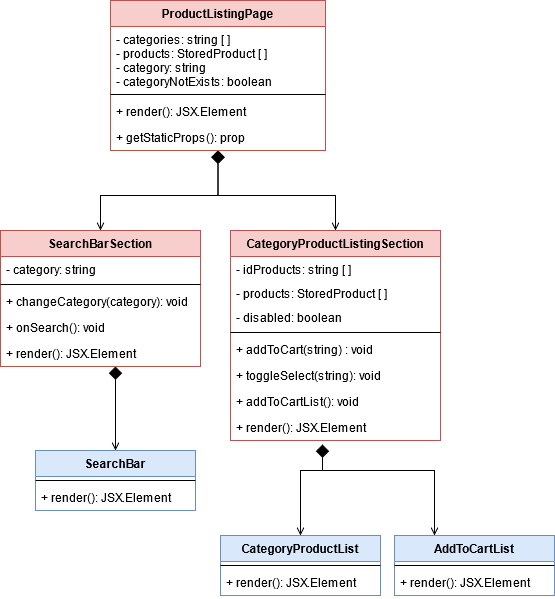
\includegraphics[scale=0.50]{res/Architettura/Frontend/img/plp}\\
\caption{Front-end\textsubscript{G} products listing page component diagram}
\end{figure}

\begin{figure}[H]
\centering
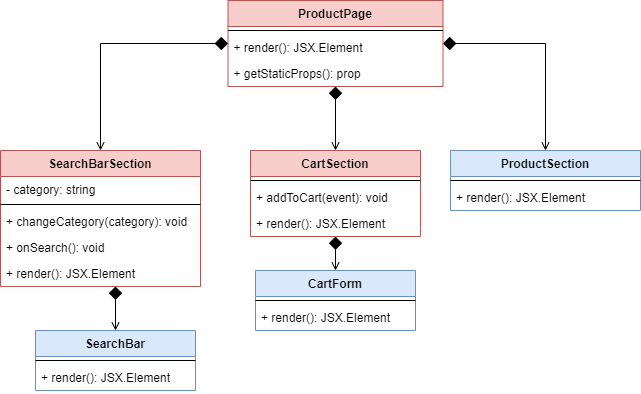
\includegraphics[scale=0.50]{res/Architettura/Frontend/img/pdp}\\
\caption{Front-end\textsubscript{G} product details page component diagram}
\end{figure}

\begin{figure}[H]
\centering
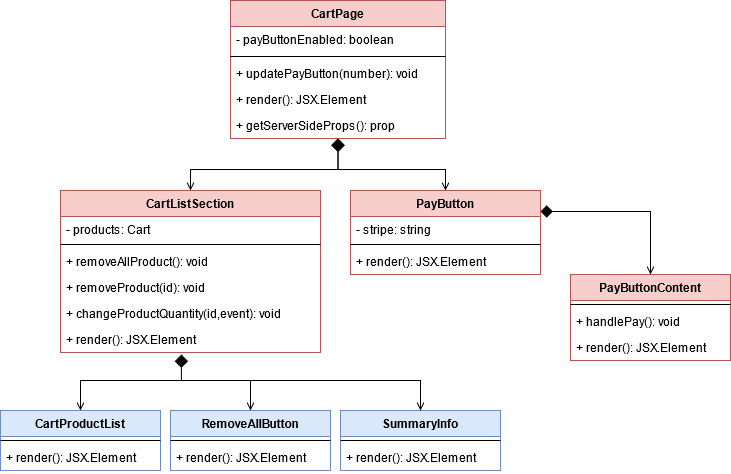
\includegraphics[scale=0.50]{res/Architettura/Frontend/img/cart}\\
\caption{Front-end\textsubscript{G} cart page component diagram}
\end{figure}

\begin{figure}[H]
\centering
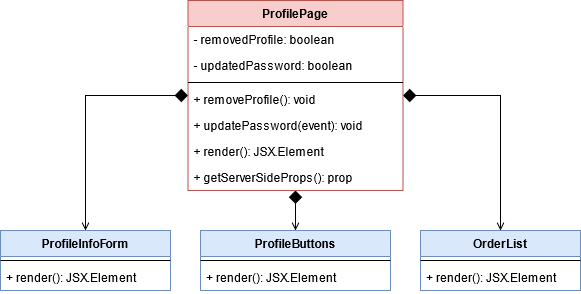
\includegraphics[scale=0.50]{res/Architettura/Frontend/img/profile}\\
\caption{Front-end\textsubscript{G} profile page component diagram}
\end{figure}

\begin{figure}[H]
\centering
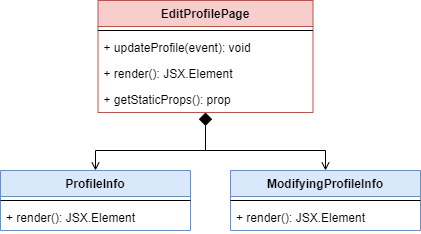
\includegraphics[scale=0.50]{res/Architettura/Frontend/img/editProfile}\\
\caption{Front-end\textsubscript{G} edit profile page component diagram}
\end{figure}

\begin{figure}[H]
\centering
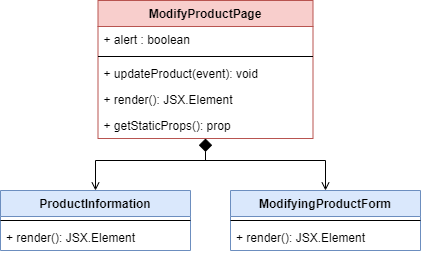
\includegraphics[scale=0.50]{res/Architettura/Frontend/img/modifyProduct}\\
\caption{Front-end\textsubscript{G} edit product page component diagram}
\end{figure}

\begin{figure}[H]
\centering
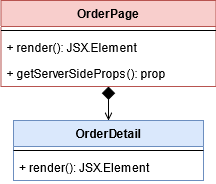
\includegraphics[scale=0.50]{res/Architettura/Frontend/img/order}\\
\caption{Front-end\textsubscript{G} order details page component diagram}
\end{figure}

\begin{figure}[H]
\centering
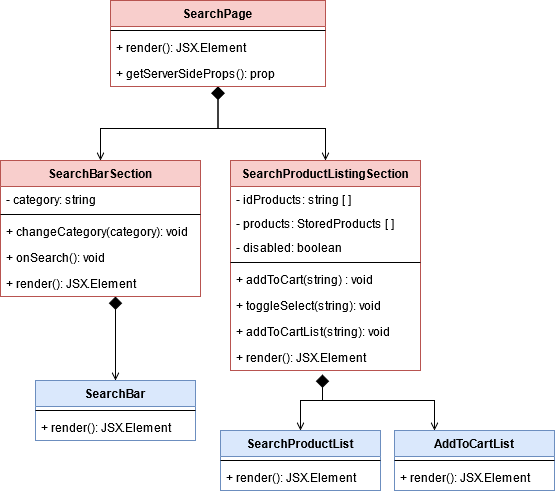
\includegraphics[scale=0.50]{res/Architettura/Frontend/img/search}\\
\caption{Front-end\textsubscript{G} search page component diagram}
\end{figure}


\newpage
\subsection{Services}
This part of the architecture lets the \textit{EmporioLambda} Front-end module retrieve or send data to the \textit{EmporioLambda} Back-end module. Services can be found inside the \textit{pages/api/Services} of the Front-end module.\\
Each service has the following composition:
\begin{itemize}
\item a Fetcher class which contains an URL generated with the pulled enviroment variables. The constructor requires the name of the function to will be called in the Back-end;
\item a getJSONResponse function which tries to make an API call to the Back-end and return the response. The return type is a Promise, as this is an asyncronous operation;
\item a getLambdaResponse function which accepts the following parameters:\begin{itemize}
\item a string which indicates the function name you want to call in your Back-end; 
\item a string which indicates the type of the call you want to do (GET, POST, PUT...);
\item a string containing the token of the current session; 
\item a string containing the parameters needed for the API call. 
\end{itemize} 
This function creates a new Fetcher object and execute the getJSONResponse method. This is the function you must call in your services.
\end{itemize}

\newpage
\subsubsection{Types}
Service calls usually return data in the JSON format. Javascript\textsubscript{G} and Typescript\textsubscript{G} are able to convert the JSON\textsubscript{G} format into a class object.\\
Because of this, the \textit{EmporioLambda} Front-end\textsubscript{G} module uses many not-primitive interfaces and classes in order to correctly convert the received JSON\textsubscript{G} data. These classes can be found inside the src/objects folder. To send data, you can use the JSON.stringify function which converts an object passed as parameter into a JSON\textsubscript{G} format string.\\Here's a class diagram that shows these classes and their dependencies between each other:
\vspace{0.5cm}
\begin{figure}[H]
\centering
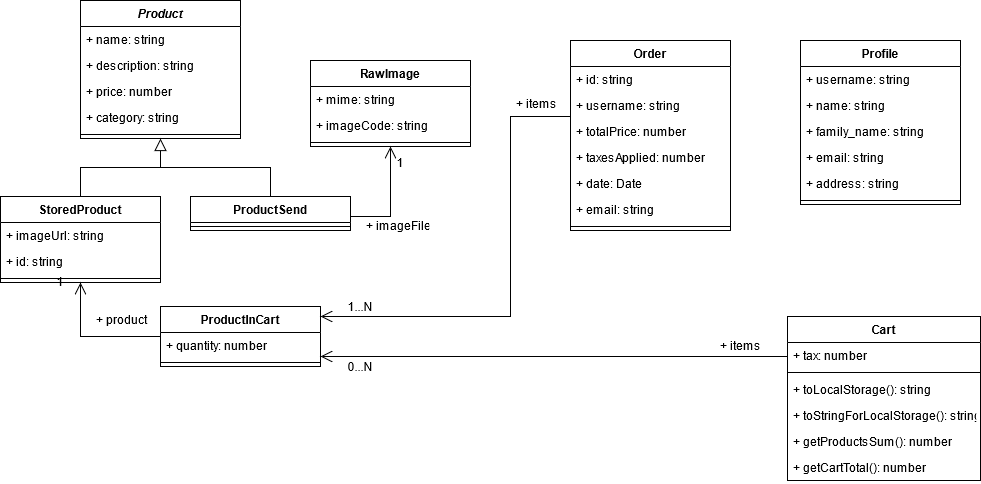
\includegraphics[scale=0.45]{res/Architettura/Frontend/img/class_frontend_types}\\
\caption{Diagram of the classes and types used in the Front-end\textsubscript{G} module}
\end{figure}
\newpage